\documentclass[10pt]{article}

\usepackage[T1]{fontenc}
\usepackage[margin=1in]{geometry}
\usepackage{setspace}
\usepackage{hyperref}
\usepackage{longtable}
\usepackage{titlesec}
\usepackage{listings}
\usepackage{xcolor}
\usepackage{graphicx}
\usepackage{booktabs}
\usepackage{enumitem}
\usepackage{cite}
\setlist{noitemsep, topsep=3pt, partopsep=0pt}

\setstretch{1.15}

\titleformat{\section}{\normalfont\Large\bfseries}{\thesection}{1em}{}
\titleformat{\subsection}{\normalfont\large\bfseries}{\thesubsection}{1em}{}
\titleformat{\subsubsection}{\normalfont\normalsize\bfseries}{\thesubsubsection}{1em}{}

\lstset{
  basicstyle=\ttfamily\small,
  breaklines=true,
  frame=single,
  backgroundcolor=\color{gray!8},
  rulecolor=\color{gray!40},
}

\title{KGRAG: A Knowledge Compiler\thanks{The \emph{Knowledge Compiler}
concept and its execution are the subject of a pending patent application
(U.S.\ provisional filed). Patent Pending. }\ and Federated Retrieval Layer\\
for Ontologically Grounded Domains}

\author{Eric G. Suchanek, PhD\\
Flux-Frontiers, Liberty Township OH\\[4pt]
\small\url{https://github.com/Flux-Frontiers/KGRAG}}
\date{}

\begin{document}

\maketitle

\begin{abstract}
KGRAG is a federation and orchestration layer for structural knowledge graphs
derived from heterogeneous source domains: Python source code (PyCodeKG), natural
language documentation (DocKG), metabolic pathway data (MetaboKG), personal diary
corpora (DiaryKG), agentic memory (MemoryKG), and a growing set of formally structured
domains including legal codes, scriptural texts, and a collection of literary works
(GutenbergKG). Each backend constructs its knowledge graph from the formal structure
of its source---abstract syntax trees for code, document section and reference graphs
for text, domain ontologies for scientific data---without any language model
participation in graph construction. The upfront computational cost of this approach
is analogous to compiling a computer program; the resulting knowledge graph is a
deterministic, verifiable, and complete representation of the source domain.
Retrieval is guaranteed to be correct by construction and does not require any inference.

The central thesis of this work is that the power of structural knowledge-graph
retrieval scales directly with the formal completeness of the source domain's
ontology. Programming languages represent the ideal case: their grammars are
complete formal specifications, and the derived graph is correct by
theorem. The same principle applies to biochemical pathway schemas, statutory
hierarchies in books of law, protein data bank file formats, and the structured
hierarchies of scripture and diary. KGRAG treats all of these domains
identically through a uniform five-method adapter protocol.

The design treats the structurally derived graph as ground truth and uses
semantic embeddings strictly as an acceleration layer for locating entry points
into that graph. Graph traversal, ranking, and snippet extraction are
deterministic: identical inputs produce identical outputs, and no component of
the structural pipeline produces probabilistic results. When KGRAG output is
passed to a large language model for synthesis, the model receives verified
facts with full source provenance, not approximate embeddings. Hallucination
risk is bounded to the synthesis stage and is zero at the knowledge-retrieval
stage.

An MCP server exposes the full federated query surface---including corpus-scoped
and person-scoped operations---to any MCP-compatible AI agent. Because retrieval
is correct by construction and results are returned in domain-native vocabulary,
synthesis does not require a frontier-scale model: a mid-tier language model
with a sufficiently large context window is enough to produce grounded answers
over the packed query result.
\end{abstract}

%-------------------------------------------------------------------
\section{Introduction}
%-------------------------------------------------------------------

Large software systems accumulate knowledge in incompatible forms. Source code
encodes behavior and architecture in a machine-readable but semantically dense
notation. Documentation encodes intent, rationale, and usage patterns in prose.
Domain corpora---pathway databases, ontologies, financial models, legal codes,
scripture---encode facts in formats specific to each field. These representations
are maintained separately, queried separately, and surfaced separately; an
analyst or an AI agent that needs to understand a system must traverse all of
them and reconcile the results manually.

The standard answer is retrieval-augmented generation (RAG): embed all documents
in a vector index and retrieve the closest matches to a query. This approach
treats source code, scientific data, and legal text as undifferentiated text,
discarding the formal structure that makes those artifacts tractable. A Python
call graph cannot be derived from a vector search; neither can a metabolic
pathway traversal, a statutory cross-reference chain, or a protein bond
topology. Vector retrieval approximates relevance; it does not expose structure.

An alternative, exemplified by GraphRAG~\cite{edge2024graphrag}, is to use a
language model to extract a knowledge graph from unstructured text. This
recovers some structure, but the structure is inferred rather than derived:
entity extraction is probabilistic, edges may be hallucinated, and the resulting
graph cannot be independently verified against any formal source.

KGRAG takes a different approach, grounded in a fundamental observation about
knowledge domains.

\subsection{The Ontology Principle}

The power of structural knowledge-graph retrieval scales directly with how
well-defined the ontology of the source domain is. A \emph{well-defined
ontology} is one where the entities, their relationships, and the rules
governing those relationships are formally specified---not inferred, not
approximated, but written down and enforced by construction.

Programming languages represent the ideal case. Python's grammar is a complete
formal specification; every function, class, import, and call site is expressed
in that grammar; and a deterministic parser can extract every structural
relationship without any inference. The derived call graph is not an
approximation---it is a theorem about the source code. The same property holds,
to varying degrees, across a surprising breadth of domains:

\begin{table}[h]
\centering
\caption{Knowledge graph domains supported by KGRAG. Bold rows indicate fully implemented adapters.}
\label{tab:domains}
\begin{tabular}{lll}
\toprule
Domain & Formal structure & KG kind \\
\midrule
\textbf{Python source code} & \textbf{Abstract syntax tree} & \textbf{\texttt{code}} \\
\textbf{Markdown / RST documentation} & \textbf{Document parse tree, hyperlinks} & \textbf{\texttt{doc}} \\
\textbf{Biochemical pathways} & \textbf{Reaction schemas (KEGG, BioCyc)} & \textbf{\texttt{meta}} \\
Protein structures & PDB file format (ATOM, SEQRES) & \texttt{pdbfile} \\
Disulfide bond families & Bond topology from PDB coordinates & \texttt{disulfide} \\
Books of law & Title $\rightarrow$ Chapter $\rightarrow$ Section $\rightarrow$ Clause & \texttt{legal} \\
\textbf{Diary / journal entries} & \textbf{Document structure + temporal order} & \textbf{\texttt{diary}} \\
Scripture / verse & Book $\rightarrow$ Chapter $\rightarrow$ Verse, cross-refs & \texttt{verse} \\
Episodic memory & Temporal event graphs & \texttt{memory} \\
Personal knowledge & Biographical and relational graphs & \texttt{person} \\
\textbf{Conversational memory} & \textbf{Turn/topic/task graph (live session)} & \textbf{\texttt{agent}} \\
\textbf{File system tree} & \textbf{Directory/file/module/dependency graph} & \textbf{\texttt{filetree}} \\
\bottomrule
\end{tabular}
\end{table}

In every case, the formal structure of the source \emph{is} the ontology, and a
knowledge graph derived from it carries the same correctness guarantees as the
source itself. This is the foundational principle of KGRAG: build knowledge
graphs from formal structure, and the graphs are correct by construction.

\subsection{The Unstructured Case: Deterministic NLP Enrichment}

Not every domain offers a complete formal grammar. Prose---technical
documentation, journals, correspondence, literary works---typically carries
only a lightweight document hierarchy (Markdown headings, paragraph breaks,
list nesting) and must recover the rest of its structure from the surface
form of the text. KGRAG handles such domains by replacing formal parsing with
\emph{deterministic NLP enrichment}: spaCy for tokenisation, named-entity
recognition, and noun-phrase extraction; lexical co-occurrence analysis for
topic clustering; structural overlap heuristics for cross-document references.
The pipeline is still deterministic, still LLM-free, and still emits
verifiable provenance for every node and edge---but the resulting graph is an
enrichment of the source rather than a theorem about it.

This is the second pillar of the design and the principal differentiator from
inference-based systems: where formal structure exists, KGRAG extracts it
exactly; where it does not, KGRAG recovers what deterministic linguistic
analysis can yield. The two regimes coexist in the federation behind one
adapter interface, and neither relies on a language model to construct the
graph.

\subsection{Contributions}

The contribution of this paper is not a new graph construction algorithm but a
new level of abstraction above existing single-domain tools: a uniform
federation layer, termed a \emph{knowledge compiler}, that makes heterogeneous
structural knowledge graphs queryable as a single unified corpus. Specifically:

\begin{enumerate}
  \item A five-method adapter protocol (\texttt{KGAdapter}), implemented
    inside kgrag as one thin wrapper class per domain, that fully decouples
    the federation layer from each backend. The wrapped domain libraries
    have no dependency on kgrag and have evolved independently against this
    stable contract; new domains are added by writing one wrapper class with
    no changes to the orchestrator, registry, CLI, or MCP server.
  \item A corpus abstraction grouping multiple KG instances for scoped federated
    queries, and a person corpus abstraction extending this with personal metadata.
  \item A complete MCP server exposing registry, corpus, and person tools to
    AI agents.
  \item A demonstration that structural KG retrieval followed by language model
    synthesis eliminates hallucination at the knowledge layer, bounding risk to
    the synthesis stage alone.
  \item A snapshot system enabling \emph{differential queries}: what changed
    between two compiled states of a knowledge graph, and what new knowledge
    entered a corpus over a given interval.
  \item An incremental ingestion pipeline with diversity-preserving temporal
    sampling and resumable state, enabling progressive compilation of large
    corpora without blocking queries.
\end{enumerate}

%-------------------------------------------------------------------
\section{Design Principles}
%-------------------------------------------------------------------

Six principles govern the design of KGRAG and its backend modules.

\begin{enumerate}

\item \textbf{Derived structure is authoritative.}
  Knowledge graphs are extracted from formal sources---ASTs, document parse
  trees, ontological schemas---by deterministic programs. The graph is not a
  model of the source; it \emph{is} the source, represented relationally.
  Embeddings are derived from it and are disposable.

\item \textbf{Semantics accelerate; structure decides.}
  Vector search locates entry points. Graph traversal determines what is
  returned. The two phases are explicit, separable, and independently tunable.
  A change to the embedding model affects which seeds are selected; a change to
  the hop count or edge filter affects traversal depth. Neither affects the
  structural layer.

\item \textbf{Every result is traceable.}
  Every node carries a stable identifier encoding its origin: file path and
  qualified name for code nodes, document path and section offset for
  documentation nodes. Every snippet is extracted from a verified location.
  Nothing enters a result without a source address.

\item \textbf{Determinism over approximation.}
  Given identical inputs, the system produces identical outputs. Ranking is
  computed by a deterministic composite key. There are no stochastic components
  in the structural or traversal layers.

\item \textbf{Generality through protocol.}
  The federation layer depends on an abstract adapter interface, not on any
  specific backend. Adding a new knowledge domain requires implementing five
  methods; the orchestrator, registry, CLI, and MCP server require no changes.

\item \textbf{Independence from language models.}
  The build pipeline, query engine, graph traversal, ranking, snippet
  extraction, and analysis tools all run locally without any language model
  call. A downstream language model may consume the output, but it plays no
  role in producing it.

\end{enumerate}

%-------------------------------------------------------------------
\section{Architecture Overview}
%-------------------------------------------------------------------

The system is organized into five abstraction layers, each with a single
responsibility and depending only on layers below it. Figure~\ref{fig:layers}
shows their arrangement.

\begin{figure}[h]
\centering
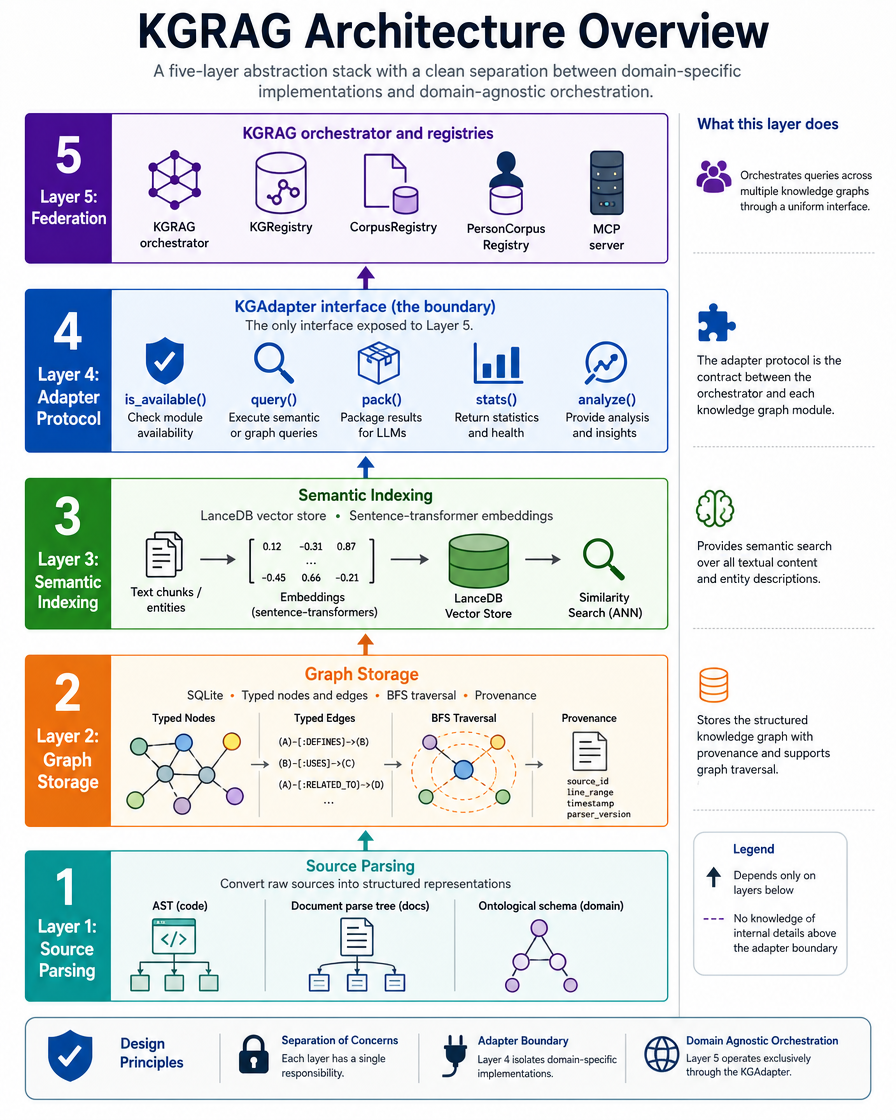
\includegraphics[width=0.68\textwidth,keepaspectratio]{../assets/kgrag_arch.png}
\caption{KGRAG abstraction layers. Each layer depends only on those below it.
The adapter protocol at Layer~4 is the boundary between domain-specific and
domain-agnostic components: everything above it is uniform across domains;
everything below it is domain-defined.}
\label{fig:layers}
\end{figure}

Layers~1--3 are implemented independently by each knowledge graph module and
are hidden behind the Layer~4 boundary. Layer~5 operates exclusively through
the \texttt{KGAdapter} interface and has no knowledge of any module's internal
representation.

%-------------------------------------------------------------------
\section{Layer 1: Source Parsing}
%-------------------------------------------------------------------

Each knowledge graph module derives its graph from the formal structure of its
source domain. Six domains are currently wrapped in kgrag with full adapters:
code (PyCodeKG), documentation (DocKG), metabolic pathways (MetaboKG), diary
corpora (DiaryKG), conversational memory (AgentKG), and file system trees
(FTreeKG). Stub adapters provide the protocol boundary for six further domains
under active development: \texttt{pdbfile}, \texttt{disulfide}, \texttt{legal},
\texttt{verse}, \texttt{memory}, and \texttt{person}.

\subsection{Python Codebase Parsing (PyCodeKG)}

\texttt{PyCodeKG.extract()} performs three deterministic AST passes over all
\texttt{.py} files in a repository. Pass~1 extracts definitions and emits
structural edges: \texttt{CONTAINS} (module to class, class to method),
\texttt{IMPORTS} (module-level import relationships), and \texttt{INHERITS}
(class to base class). Pass~2 extracts the call graph, emitting \texttt{CALLS}
edges annotated with call-site evidence: the line number and expression text of
each call site, extracted directly from the AST node.

Pass~3 runs a data-flow visitor (\texttt{PyCodeKGVisitor}) that extends
\texttt{ast.NodeVisitor} to emit three additional edge types per function:
\texttt{READS} (variable consumption), \texttt{WRITES} (variable assignment),
and \texttt{ATTR\_ACCESS} (attribute access on a named object). These capture
intra-function data movement without requiring execution or type inference.

A post-build step, \texttt{resolve\_symbols()}, name-matches every unresolved
call target (represented as a \texttt{sym:} stub node) against all first-party
definitions and writes \texttt{RESOLVES\_TO} edges. This enables cross-module
fan-in queries: given a function, which functions in other modules call it?

All nine declared edge relations---\texttt{CONTAINS}, \texttt{IMPORTS},
\texttt{INHERITS}, \texttt{CALLS}, \texttt{READS}, \texttt{WRITES},
\texttt{ATTR\_ACCESS}, \texttt{DEPENDS\_ON}, and \texttt{RESOLVES\_TO}---are
derived from syntax. No relation is inferred.

\subsection{Document Corpus Parsing (DocKG)}

DocKG is the canonical example of the unstructured-text regime. The Markdown
heading hierarchy and link graph supply the structural skeleton; the prose
body inside each section is processed by a multi-pass NLP pipeline. Pass~1
chunks each section into overlapping windows and applies spaCy for
tokenisation, named-entity recognition, and noun-phrase extraction. Pass~2
performs lexical co-occurrence and overlap analysis to cluster keywords into
topics. Six node kinds are emitted (\texttt{document}, \texttt{section},
\texttt{chunk}, \texttt{entity}, \texttt{keyword}, \texttt{topic}) connected
by eight edge types. No language model participates; every node carries a
deterministic origin (file path, section path, character span) and every edge
records its source. DiaryKG reuses the same pipeline and adds a temporal
axis: dated entries become time-ordered chunks with explicit \texttt{PRECEDES}
edges and date-anchored seeds for temporal queries.

\subsection{Domain Corpus Parsing (MetaboKG and Beyond)}

MetaboKG wraps a domain-specific backend---initially targeting metabolic
pathway databases---via the same \texttt{KGAdapter} interface. DiaryKG parses
dated diary entries (plain text or PDF) into timestamped chunk graphs with
temporal edges. AgentKG builds a live conversational memory graph from session
turn sequences, emitting Turn, Topic, Task, and Summary nodes that are
queryable across sessions. The parsing strategy of each backend is
domain-defined; the interface contract is uniform. A biochemical pathway
graph derived from KEGG, a diary corpus derived from plain-text journal
files, a conversational session derived from turn sequences, and---once the
corresponding compilers are complete---a protein topology derived from PDB
ATOM records, a legal code derived from statutory filings, and a verse
graph derived from scripture chapter/verse structure will all surface
identically to the federation layer.

This uniformity is not accidental. It is the central claim of the ontology
principle: \emph{where formal structure exists, structural parsing produces
graphs with the same correctness guarantees as the source, and the federation
layer need not know which domain it is querying.}

%-------------------------------------------------------------------
\section{Layer 2: Graph Storage}
%-------------------------------------------------------------------

All modules persist their graphs to SQLite in a two-table schema: a
\texttt{nodes} table and an \texttt{edges} table. Node records carry a stable
string identifier, a kind, a name, and a JSON metadata blob. Edge records carry
source node ID, relation name, destination node ID, and optional JSON evidence.

Node identifiers are deterministically constructed from kind, source path, and
qualified name. For example: \texttt{m:src/kg\_rag/orchestrator.py:KGRAG.query} (methods use the \texttt{m:} prefix; module-level functions use \texttt{fn:}).
This means a node ID is stable across rebuilds as long as the source does not
move, and it is human-readable and directly linkable to the source.

The key traversal primitive is \texttt{expand(seed\_ids, hop, rels)}: a bounded
breadth-first search from a set of seed nodes, following a specified set of edge
relations up to a configurable hop limit. Each reached node is annotated with
\texttt{ProvMeta}: its minimum hop distance from any seed and the originating
seed node ID. Provenance travels with every result.

%-------------------------------------------------------------------
\section{Layer 3: Semantic Indexing}
%-------------------------------------------------------------------

\texttt{SemanticIndex} reads nodes from a \texttt{GraphStore}, constructs a
canonical text document for each node (name plus available descriptive text),
embeds them using a sentence-transformer model, and stores the vectors in
LanceDB. The index is derived from the SQLite graph and is fully disposable.
Its only function is to rank nodes by semantic similarity to a query string,
producing a short list of seed node IDs for the subsequent structural traversal.

The separation is intentional and load-bearing. If the embedding model is
replaced, the new index will select different seeds; the traversal from those
seeds will still follow the same structural edges and produce structurally
correct results. The accuracy of the structural layer does not depend on the
quality of the embedding model.

\subsection{The Compilation Cost: Paid Once}

Embedding is the computationally expensive phase of the KGRAG pipeline, and it
is worth making this explicit. Encoding tens of thousands of nodes into
high-dimensional vectors using a sentence-transformer model is a non-trivial
compute task; for a large diary corpus or a full legal code, it may require
minutes to hours on CPU hardware.

This is not a deficiency. It is an instance of a well-understood engineering
trade-off: the compiler trade-off. Compiling a large Fortran simulation suite
may take tens of minutes, but the resulting binary executes in milliseconds and
may be run any number of times without recompilation. The compile cost is
amortised across every subsequent execution.

KGRAG applies the same trade-off. The \emph{build} step---parse, extract,
store, embed---is the compilation. Each subsequent \emph{query} is execution:
instantaneous, deterministic, and repeatable. A federated query over a
codebase of $\sim$100\,k lines runs in under one second. The embedding cost
was paid during build, once, and is not paid again until the corpus changes.

This framing also clarifies what the compiled artefact represents. A compiled
binary is the source program, in executable form. The compiled knowledge
graph---SQLite nodes and edges plus LanceDB vectors---\emph{is} the corpus, in
queryable form. Just as one does not re-read the source to run the program,
one does not re-parse the corpus to answer a query. The structure is already
there, addressable in constant time.

%-------------------------------------------------------------------
\section{Layer 4: The Adapter Protocol}
%-------------------------------------------------------------------

\texttt{KGAdapter} is an abstract base class with five abstract methods. It
is the internal contract between kgrag's federation layer and the per-domain
wrapper classes that live alongside it in the kgrag source tree (under
\texttt{src/kg\_rag/adapters/}). For each supported domain, kgrag holds one
thin adapter subclass that implements the five-method contract by translating
into calls on the wrapped library's native API.

The wrapped libraries themselves---\texttt{pycode\_kg}, \texttt{doc\_kg},
\texttt{diary\_kg}, \texttt{agent\_kg}, \texttt{metabokg}---are independent
packages that have no compile- or run-time dependency on kgrag. They are
installable and usable standalone, expose their own domain-native interfaces,
and have evolved separately against this stable contract: kgrag depends on
them, never the reverse. This dependency inversion is the load-bearing
architectural choice. Domain specialists ship new compilers (or update
existing ones) without touching the federation layer; the federation layer
admits a new domain by adding one wrapper class without touching any compiler.

\begin{lstlisting}[language=Python]
class KGAdapter(ABC):
    def __init__(self, entry: KGEntry, embedder=None) -> None: ...

    @abstractmethod
    def is_available(self) -> bool: ...

    @abstractmethod
    def query(self, q: str, k: int = 8,
              min_score: float = 0.0,
              semantic_floor: float = 0.0) -> list[CrossHit]: ...

    @abstractmethod
    def pack(self, q: str, k: int = 8,
             context: int = 5,
             semantic_floor: float = 0.0) -> list[CrossSnippet]: ...

    @abstractmethod
    def stats(self) -> dict[str, Any]: ...

    @abstractmethod
    def analyze(self) -> str: ...

    # Concrete template method -- not abstract; subclasses override
    # _collect_snapshot_metrics() to add domain-specific fields.
    def snapshot(self, version: str,
                 label: str | None = None) -> dict[str, Any]: ...

    # Internal -- strips domain-specific fields; used by the orchestrator
    # to aggregate graph-size metrics uniformly across all KG kinds.
    def _graph_stats(self) -> dict[str, int]: ...
\end{lstlisting}

The \texttt{snapshot} method is a \emph{concrete template method} on the base
class: it builds a standard envelope (version string, ISO~8601 UTC timestamp,
node count, edge count) and merges in any domain-specific data returned by the
subclass hook \texttt{\_collect\_snapshot\_metrics()}. Subclasses extend the
snapshot by overriding only that hook, not \texttt{snapshot} itself. The
\texttt{\_graph\_stats} helper is likewise concrete: it strips all
domain-specific keys from \texttt{stats()} and normalises counts to integers so
the orchestrator can aggregate graph-size totals uniformly across heterogeneous
KG kinds without being confused by domain-specific fields such as
\texttt{reaction\_count} or \texttt{chunk\_count}.

A \texttt{StubKGAdapter} base class provides a graceful default implementation
for domains whose backing library has not yet been released. Stub adapters
return empty results from \texttt{query} and \texttt{pack}, report
\texttt{status: unavailable} from \texttt{stats}, and produce a structured
unavailability notice from \texttt{analyze}. This allows new domains to be
registered, grouped into corpora, and included in federated queries before
their compilers are complete; they participate in the structure of the
knowledge graph but contribute no data until ready.

The adapter protocol defines the boundary between the universal and the
specific. Everything above Layer~4 is domain-agnostic.

%-------------------------------------------------------------------
\section{Layer 5: Federation}
%-------------------------------------------------------------------

\subsection{Registry}

\texttt{KGRegistry} maintains a persistent SQLite table of \texttt{KGEntry}
records. Each entry records the KG instance name, its kind, the repository
root, paths to its SQLite and LanceDB databases, the module version, and a
JSON metadata blob. Registration is performed once per project; subsequent
queries consult the registry to locate all known KG instances.

\subsection{Corpus and Person Corpus Registries}

Two higher-level registries group KG instances for scoped federated queries.

\texttt{CorpusRegistry} maintains a \texttt{corpora} table in the same SQLite
file. A \texttt{CorpusEntry} is a named list of \texttt{KGEntry} UUIDs with an
optional description and tags. Corpus operations (\texttt{query\_corpus},
\texttt{pack\_corpus}, \texttt{stats\_corpus}) resolve the UUID list to
\texttt{KGEntry} objects and dispatch to the same adapter machinery as
global queries.

\texttt{PersonCorpusRegistry} extends this with personal metadata: birth year,
birth date, address, email, phone, and free-form notes. A
\texttt{PersonCorpusEntry} is the natural grouping for all KGs relevant to an
individual---diary entries, memory graphs, documents, code, verse, correspondence.
Person queries fan out over all of the person's KGs:

\begin{lstlisting}
kgrag corpus person query "Eric Suchanek" \
    "disulfide bond research 2019"
\end{lstlisting}

\subsection{Orchestrator}

\texttt{KGRAG} is the cross-KG orchestrator. On each query, it:

\begin{enumerate}
  \item Retrieves all entries from the registry, optionally filtered by kind.
  \item For each entry, instantiates (or retrieves from cache) the corresponding
    \texttt{KGAdapter} and verifies availability.
  \item Dispatches the query string to each available adapter in sequence,
    collecting \texttt{CrossHit} or \texttt{CrossSnippet} lists.
  \item Merges all results into a single list and sorts by score descending.
  \item Returns a typed result object with the merged list and per-KG metadata.
\end{enumerate}

The dispatch loop is deliberately simple. Individual adapter calls are
independent; a failure in one does not abort the others. Stub adapters (for
domains whose libraries are not yet available) return empty lists and are
silently skipped.

\subsection{Result Types}

\texttt{CrossQueryResult} carries the merged hit list, the per-KG breakdown,
the total hit count, and the number of KGs that were actually queried.

\texttt{CrossSnippetPack} carries the merged snippet list and an approximate
token count for budget-aware context assembly. \texttt{CrossSnippetPack.render()}
produces a single LLM-ready string with section headers identifying each
snippet's source domain, KG name, file path, and line span.

%-------------------------------------------------------------------
\section{Query Execution}
%-------------------------------------------------------------------

A federated query executes as follows at each participating adapter:

\begin{enumerate}
  \item \textbf{Semantic seeding.} The query string is embedded and used to
    retrieve $k$ seed nodes from LanceDB.
  \item \textbf{Structural expansion.} \texttt{GraphStore.expand()} performs
    BFS from the seed IDs, following a specified set of edge relations up to
    a configurable hop limit. Each reached node is annotated with
    \texttt{ProvMeta}.
  \item \textbf{Ranking.} Nodes are ranked by a deterministic composite key:
    hop distance (ascending), seed embedding distance (ascending), node kind
    priority, node ID as tiebreaker.
  \item \textbf{Deduplication.} For snippet queries, nodes are deduplicated by
    file and source span.
  \item \textbf{Snippet extraction.} Source text is extracted at each retained
    node's verified path and line span, with a configurable context window.
\end{enumerate}

After each adapter completes, the orchestrator merges results and performs a
final global sort by score. End-to-end latency for a federated query over a
codebase of $\sim$100\,k lines is typically under one second on commodity hardware.

\subsection{Ontology-Aware Result Enrichment}

Every adapter returns results in the proper semantic vocabulary of its domain,
not the raw internal identifiers of the underlying graph. A MetaboKG query
does not surface opaque reaction codes such as \texttt{R00200}; it returns
the catalysing enzyme name, the reaction in human-readable form
(\emph{phosphoenolpyruvate $\rightarrow$ pyruvate}), the EC number, and the
pathway membership. A PyCodeKG query does not surface internal hashes; it
returns qualified names such as \texttt{KGRAG.query} together with the file
path and line span. A DocKG query returns the document title and section
heading path (\emph{``Architecture~$\rightarrow$~Layer~4: Adapter Protocol''})
rather than chunk offsets. A DiaryKG query returns the entry date and any
extracted title (\emph{``1665-09-04 — fire reaches Pudding Lane''}) instead
of a row index. An AgentKG query returns the conversational turn with its
topic and task labels rather than a session-internal turn number.

The internal identifiers remain available---every result carries its stable
node ID, which a downstream language model may use as a deterministic
citation key or pass back through any KGRAG tool for verification---but the
surface presentation is the form a domain expert would write or read. The
federation layer never collapses domain-specific naming into a generic
representation; each adapter is responsible for restoring the vocabulary of
its source domain on output. The result is dual-audience: immediately legible
to humans, semantically meaningful to language models, and precisely
addressable for verification against the original artefact.

%-------------------------------------------------------------------
\section{Grounded Synthesis and the Hallucination Bound}
%-------------------------------------------------------------------

When the output of a KGRAG federated query is passed to a large language model
for synthesis, the combination constitutes what we term \emph{Structural
KG-RAG}~\cite{suchanek2025codekg}: knowledge-graph-augmented generation in which
the knowledge graph was not itself produced by a language model.

Every piece of context in the synthesis prompt carries:
\begin{itemize}
  \item A stable node identifier encoding its source address
  \item A source file path and line span
  \item A deterministically computed relevance score
  \item The actual source text
\end{itemize}

The language model is presented with \emph{facts}, not \emph{embeddings}. Its
role is synthesis---connecting, explaining, summarizing---not construction of
the knowledge itself. The critical consequence is that \textbf{hallucination
risk at the knowledge-retrieval stage is zero.} The model cannot fabricate a
PyCodeKG function call that is not in the graph, because the graph was derived
from the AST; it cannot invent a MetaboKG reaction edge absent from the
pathway schema; it cannot surface a DocKG entity that spaCy did not extract
from a recorded character span, nor a DiaryKG entry on a date that does not
exist in the corpus.

Hallucination risk is confined to the synthesis stage alone---where the model
may reason incorrectly over correct facts. This risk is substantially lower and
is addressed by standard techniques (chain-of-thought, self-consistency,
re-querying). The knowledge foundation is correct by construction in the
formal domains and verifiably-sourced in the NLP-derived domains; in neither
case can the model invent facts that are absent from the underlying source.

This is the decisive advantage of structural KG-RAG over inference-based
approaches: the correctness guarantee is unconditional with respect to the
structural layer and does not depend on prompt engineering, model scale, or
retrieval quality.

\subsection{Modest Models, Generous Context}

A practical consequence of the enrichment described above is that the
synthesis model does not need to be large. Conventional RAG pipelines lean on
frontier-scale models in part to compensate for noisy retrieval: the model
must guess which fragments are relevant, reconcile contradictory snippets,
and infer entity identity from surface similarity. KGRAG removes that work
upstream. The packed context is already deduplicated, ranked deterministically,
labelled with domain-native names, and tagged with verifiable provenance.
Synthesis collapses to summarisation and exposition over facts that are
already correct.

A mid-tier model with a generous context window---enough to hold the full
snippet pack of a federated query and the user's question---is sufficient
for high-quality answers. The bottleneck shifts from model capability to
context capacity: how much of the compiled corpus can be presented at once.
This inverts the usual deployment economics. Rather than paying for the
largest available model on every query, KGRAG users can run a smaller model
with a long context for routine work and reserve frontier-scale synthesis
for genuinely difficult reasoning over the same already-correct facts.

%-------------------------------------------------------------------
\section{Snapshot System and Differential Queries}
%-------------------------------------------------------------------

Knowledge graphs change as their source corpora evolve. The snapshot system
captures \texttt{SnapshotMetrics} at each build or ingestion run, keyed by the
git tree hash produced by \texttt{git write-tree}. A \texttt{Snapshot} record
carries the tree hash, branch name, ISO~8601 timestamp, module version, a
\texttt{SnapshotMetrics} struct (node counts, edge counts, coverage score, issue
count), and \texttt{SnapshotDelta} fields comparing against the immediately
preceding and baseline snapshots.

The snapshot history provides a longitudinal record of graph evolution. More
importantly, it enables a class of queries that is impossible with a conventional
vector index: \emph{differential queries} over the knowledge graph.

Consider two questions that are straightforward to answer once snapshots exist
but are unanswerable without them:

\begin{enumerate}
  \item \emph{How has the Pepys corpus changed since last week?} \\
    Compare the two nearest snapshots by tree hash. The delta carries exact node
    and edge counts added and removed, the set of new topic labels that entered
    the corpus, and the change in semantic coverage score. This is
    \texttt{pycodekg snapshot diff} (or \texttt{dockg snapshot diff}) operating
    on two snapshot keys; each backend CLI exposes this command directly.

  \item \emph{What new ideas have entered the Pepys corpus this month?} \\
    Execute a federated query against both snapshots, compute the set difference
    of the top-$k$ results, and the remainder is the new knowledge. New nodes
    that did not exist in the earlier snapshot and rank highly in the current
    one represent ideas that have entered the compiled corpus. This is
    \emph{differential federated search}: the same query, two compiled states,
    a structural diff.
\end{enumerate}

These capabilities are direct consequences of the compilation model. A raw
vector index can be updated incrementally, but its history is not addressable;
there is no mechanism to query ``the index as it was on Tuesday.'' The compiled
knowledge graph, stored in SQLite and keyed by git tree hash, is fully
addressable at any point in its history.

\subsection{Incremental Ingestion with Temporal Diversity}

Large corpora may not be fully ingestable in a single run. KGRAG addresses
this with a diversity-preserving batch selection algorithm. When
\texttt{batch\_size} is set, the ingestion pipeline clusters all available
entries in a normalised feature space encoding temporal position, content
length, lexical density, and named-entity profile, then selects the
centroid-nearest entry from each cluster. A batch of 200 entries from a
10,000-entry diary corpus will span the full temporal range and all discoverable
themes of that corpus, not merely its beginning.

A state manager tracks processed entry indices. Subsequent runs with
\texttt{--resume} load this state, skip already-ingested entries, and select a
fresh diverse batch from the remainder. The corpus is queryable throughout:
an index built from 200 representative entries already covers the semantic space
of the full corpus at reduced density. Density increases with each run until
full ingestion is achieved.

%-------------------------------------------------------------------
\section{MCP Integration}
%-------------------------------------------------------------------

An MCP server wraps the \texttt{KGRAG} orchestrator and exposes a complete
tool surface to any MCP-compatible AI agent. Tools are organized into three
groups.

\textbf{Registry tools:}
\begin{center}
\begin{tabular}{ll}
\toprule
Tool & Function \\
\midrule
\texttt{kgrag\_stats()} & Registry summary: KG count, kinds, built status \\
\texttt{kgrag\_list([kind])} & List registered KG entries, optionally filtered \\
\texttt{kgrag\_info(name)} & Full detail for a single KG entry \\
\texttt{kgrag\_query(q, [k, kinds])} & Federated semantic query, JSON result \\
\texttt{kgrag\_pack(q, [k, kinds])} & Federated snippet pack, Markdown output \\
\bottomrule
\end{tabular}
\end{center}

\begin{sloppypar}
\textbf{Corpus tools} (\texttt{kgrag\_corpus\_list}, \texttt{kgrag\_corpus\_info},
\texttt{kgrag\_corpus\_create}, \texttt{kgrag\_corpus\_delete},
\texttt{kgrag\_corpus\_add}, \texttt{kgrag\_corpus\_remove},
\texttt{kgrag\_corpus\_query}, \texttt{kgrag\_corpus\_pack}): create and manage
named collections of KG instances and execute corpus-scoped federated queries.
\end{sloppypar}

\begin{sloppypar}
\textbf{Person tools} (\texttt{kgrag\_person\_list}, \texttt{kgrag\_person\_info},
\texttt{kgrag\_person\_create}, \texttt{kgrag\_person\_delete},
\texttt{kgrag\_person\_add}, \texttt{kgrag\_person\_remove},
\texttt{kgrag\_person\_update}, \texttt{kgrag\_person\_query},
\texttt{kgrag\_person\_pack}): create and manage person corpus entries with
personal metadata and execute person-scoped federated queries.
\end{sloppypar}

The MCP transport is \texttt{stdio}, making it compatible with Claude Code,
Kilo Code, GitHub Copilot, Cline, and Claude Desktop without additional
networking configuration.

%-------------------------------------------------------------------
\section{Comparison with Inference-Based Graph Construction}
%-------------------------------------------------------------------

GraphRAG~\cite{edge2024graphrag} is the most widely deployed system in the
vicinity of this work. Both KGRAG and GraphRAG augment retrieval with a
knowledge graph; the origin and guarantees of that graph differ substantially.

In GraphRAG, a language model extracts entities and relationships from text
documents. The graph is a product of language model inference; its correctness
is bounded by extraction prompt quality and model comprehension. Errors
introduced during extraction are silent: the system has no mechanism to verify
that an extracted relationship corresponds to anything in the source.

In KGRAG, knowledge graphs are derived from the source by deterministic
programs. A PyCodeKG \texttt{CALLS} edge exists because a call expression was
found in the AST at the recorded line number. A MetaboKG reaction edge exists
because it appears in the source pathway schema. A DocKG \texttt{MENTIONS}
edge exists because spaCy named-entity recognition matched a span in the
section text at a recorded character offset. A DiaryKG \texttt{PRECEDES} edge
exists because two entries are dated. No edge is inferred by a language model;
every edge is verified against a deterministic source address---whether that
address is an AST node, a schema row, or a character span produced by a
deterministic NLP pass.

\begin{table}[h]
\centering
\caption{Inference-based vs.\ structure-derived knowledge graph retrieval}
\label{tab:comparison}
\begin{tabular}{lll}
\toprule
Property & GraphRAG~\cite{edge2024graphrag} & KGRAG \\
\midrule
Graph source        & LLM extraction from text      & Formal source parsing \\
Graph correctness   & Probabilistic                 & Deterministic \\
Edge evidence       & NL relationship description   & Source address + line \\
LLM required to build  & Yes                        & No \\
LLM required to query  & No                         & No \\
Domain generality   & Text corpora                  & Formal-structure + NLP-enriched prose \\
Hallucination risk (KG layer) & Present             & Zero \\
Hallucination risk (synthesis) & Present            & Present (bounded) \\
Result provenance   & Document reference            & Node ID + file + line \\
Query latency       & Seconds to minutes            & Under one second (local) \\
\bottomrule
\end{tabular}
\end{table}

The two systems are not in competition for the same problem. GraphRAG is
designed for global sensemaking over large unstructured text corpora. KGRAG
is designed for structural navigation of formally specified artifacts, with a
zero-hallucination guarantee at the knowledge layer.

%-------------------------------------------------------------------
\section{Conclusion}
%-------------------------------------------------------------------

KGRAG demonstrates that structural knowledge from heterogeneous source domains
can be federated under a single uniform interface without collapsing domain
specificity into a common text representation. The adapter protocol cleanly
separates domain-specific extraction from domain-agnostic orchestration.

The central findings of this work are:

\begin{enumerate}

\item \textbf{The Ontology Principle.} The power of structural KG retrieval
  scales with how well the source domain's ontology is specified. Programming
  languages are the ideal case (PyCodeKG, full grammar); biochemical pathways
  follow with explicit reaction schemas (MetaboKG); prose corpora and journals
  carry only lightweight Markdown and temporal structure but yield to
  deterministic NLP enrichment (DocKG, DiaryKG). Where formal structure
  exists, the derived graph is correct by construction. Where it does not,
  the graph is verifiably sourced from deterministic linguistic analysis. In
  neither regime does a language model construct the graph.

\item \textbf{The Knowledge Compiler.} KGRAG is not a retrieval system that
  happens to use graphs. It is a knowledge compiler: it transforms formally
  structured source artifacts into relational representations that preserve and
  expose the structure of the originals. The compiled knowledge graph \emph{is}
  the corpus, represented for navigation.

\item \textbf{Universal Federation.} Because all domain adapters expose the
  same five-method interface, all compiled knowledge is queryable through one
  interface. The scientist, lawyer, software engineer, and biographer query the
  same system. One command, one ranking, full provenance.

\item \textbf{Zero Hallucination at the Knowledge Layer.} When KGRAG output is
  passed to a language model for synthesis, the model receives verified facts
  with source addresses. Hallucination risk is bounded to the synthesis stage
  alone and is zero at the knowledge-retrieval stage. This is an unconditional
  guarantee: it holds regardless of model scale, prompt engineering, or
  retrieval quality.

\end{enumerate}

The result is a retrieval system that is fast, auditable, and correct by
construction at the structural layer. Because the retrieved context is already
correct, deduplicated, and presented in domain-native vocabulary, synthesis
is a comparatively light task: a mid-tier language model with a generous
context window suffices for most workloads, and the largest available models
can be reserved for genuinely hard reasoning over the same already-correct
facts. The correctness guarantee holds regardless of the synthesis model's
scale, because the model receives facts rather than constructs them. That is
the ultimate power of the design.

%-------------------------------------------------------------------
\begin{thebibliography}{9}

\bibitem{edge2024graphrag}
Darren Edge, Ha Trinh, Newman Cheng, Joshua Bradley, Alex Chao, Apurva Mody,
Steven Truitt, and Jonathan Larson.
\newblock From local to global: A graph {RAG} approach to query-focused
summarization.
\newblock \emph{arXiv preprint arXiv:2404.16130}, 2024.
\newblock \url{https://arxiv.org/abs/2404.16130}

\bibitem{suchanek2025codekg}
Eric G. Suchanek.
\newblock {PyCodeKG}: Deterministic code navigation via knowledge graphs,
semantic indexing, and grounded context packing.
\newblock Technical report, Flux-Frontiers, 2025.
\newblock \url{https://github.com/Flux-Frontiers/pycode\_kg}

\bibitem{reimers2019sbert}
Nils Reimers and Iryna Gurevych.
\newblock Sentence-{BERT}: Sentence embeddings using {Siamese} {BERT}-networks.
\newblock In \emph{Proceedings of EMNLP 2019}, 2019.
\newblock \url{https://arxiv.org/abs/1908.10084}

\end{thebibliography}

\end{document}
